\documentclass{article}
\usepackage[utf8]{inputenc}
\usepackage{graphicx}
\usepackage[spanish]{babel}


\begin{document}

\begin{figure}[t!]

\includegraphics[scale=0.3]{logo_udp.PNG}
\label{fig:udplogo}
\end{figure}

\title{\textbf{{Laboratorio 7 \\ Sockets \vspace{10cm}}}}
\author{\hspace{8cm} Vicente Henriquez \\ \hspace{8cm} Franco Montenegro}
\date{\hspace{8cm} 17/11/2017}
\maketitle

\newpage
\tableofcontents

\newpage
\section{Introducción\vspace{0.5cm}}
En este informe se explicará el funcionamiento de nuestro programa, este programa se basará en todo lo aprendido a lo largo del curso redes de datos y sus respectivas ayudantías, más específicamente a la conexión entre computadores a través de sockets que refiere a una comunicación mediante flujo de datos, en este caso un computador A funcionando como Servidor-Cliente y otro computador B y/o C funcionando solo como Cliente.
Nuestro programa se basará en un clásico juego de cartas Black Jack que consiste en obtener una puntuación de 21 o lo más cercano a ello sin pasarse, donde los clientes tomarán el papel de jugadores y el servidor de crupier. 

\newpage
\section{Desarrollo\vspace{0.5cm}}
El objetivo de nuestro trabajo, luego de haber entendido el concepto de socket, es mezclar lo aprendido de dicho termino con lo programación de (en este caso) un juego, es decir, llevaremos nuestro código de socket al Black Jack y en un futuro ideal a más juegos.\newline
A continuación se presentarán los códigos primarios o base de lo que será nuestro proyecto. (Por motivos obvios no presentaremos el código completo del juego en el informe, se adjuntará en el correo y se mostrará la interfaz actual)

\begin{figure}[h!]
\centering
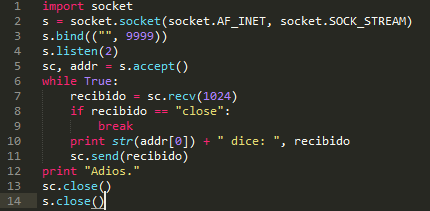
\includegraphics[scale=0.7]{server.png}
\caption{Código Servidor}
\label{fig:serv}
\end{figure}

\begin{figure}[h!]
\centering
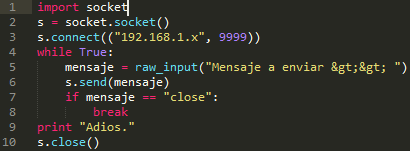
\includegraphics[scale=0.7]{client.png}
\caption{Código Cliente}
\label{fig:client}
\end{figure}

Cabe aclarar que el código base del juego Black Jack no nos pertenece, será especificado en el GitHub.(Figura \ref{fig:bj})
\newpage
\begin{figure}[h!]
\centering
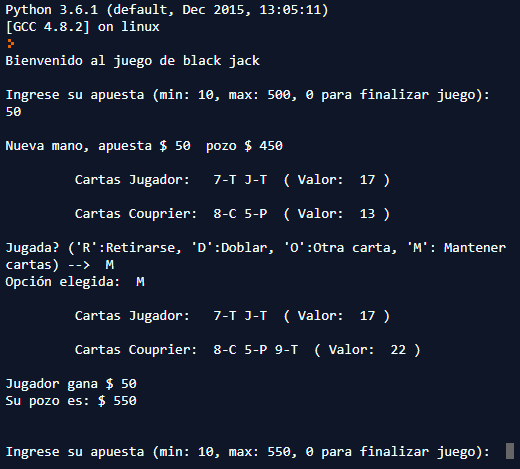
\includegraphics[scale=0.7]{Blackj.png}
\caption{Black Jack}
\label{fig:bj}
\end{figure}

Para que se pueda llevar a cabo este juego debemos tener una baraja, las representaremos como una función mediante duplas (valor, palo), declararemos los palos como una lista de C (corazones), D (diamante), T (trébol) y P (pica), para los valores numéricos de las cartas utilizaremos [A + rango del (2,11)  + J ,Q ,K] con A representando el As, por lo tanto la baraja quedaría declarada como una lista representada por valores y palos, una carta quedaría así: \\
(A,C)-> As de Corazones, y así quedaría la baraja lista.
Pero para un juego de cartas necesitamos que la baraja sea aleatoria y esto lo logramos con funciones importadas de otras librerías como import random con lo cual lograríamos una elección aleatoria de una carta y luego la removeríamos ya que no siguen en juego las cartas ya utilizadas.\\
Luego que tenemos el problema de las cartas solucionado hay que ir a las reglas del juego, en este caso un computador X hará de croupier y al mismo tiempo podrá ser utilizado como jugador conectado a máximo 2 computadores más a través de sockets, para este juego de cartas el valor de As puede ser 1 u 11, mientras J, Q, K toman el valor de 10. Una parte esencial del juego son las apuestas, en este programa uno tendrá 500 de valor inicial para apuestas y cada jugada tendrá la oportunidad de seguir apostando más o retirare.\\
Se empezará repartiendo 2 cartas a cada jugador y tendremos una función definida para el cálculo del valor de la mano, así mismo para determinar la siguiente jugada gracias a una función declarada anteriormente (def solicitar jugada) tendremos los siguientes opciones de comandos ingresados por el usuario:\\
R->Retirarse, D->doblar apuesta, O->pedir otra carta, M->mantener cartas.\\
Luego de tener esto tenemos una función que determinara cuanto es la ganancia del jugador en ronda, que se basara en cuanto aposto, si gano o perdió este turno y en caso de ganar cuanto era el pozo de ese turno.


\newpage

\section{Conclusión\vspace{0.5cm}}

Para finalizar nuestras ideas, esperamos lograr nuestro objetivo con el mejor de los éxitos, es más, sería ideal poder agregar algún otro juego a nuestra lista en el actual proyecto. La motivación y entusiasmo ante el laboratorio no ha dejado de ser la misma que el primer día, ya que el concepto de socket más allá de ser abstracto es muy interesante. 


\end{document}